\chapter{System Design and Architecture}
\label{ch:system-design}

This chapter presents the detailed architectural design of the Dynamic \qos Scheduler, including component specifications, data flow models, algorithmic formulations, and interface definitions. The design follows a layered architecture pattern with clear separation of concerns.

\section{Architectural Overview}
\label{sec:arch-overview}

\subsection{Design Principles}

The system architecture adheres to the following principles:

\begin{enumerate}[leftmargin=*]
    \item \textbf{Separation of Concerns:} Traffic classification, bandwidth scheduling, device management, and user interface are implemented as independent, loosely coupled components.
    
    \item \textbf{Reactive Design:} State changes propagate automatically through observable data streams (Kotlin StateFlow), eliminating manual synchronization.
    
    \item \textbf{Performance-First:} Critical path operations (packet parsing, token bucket consumption) are optimized for sub-millisecond execution.
    
    \item \textbf{Fail-Safe Operation:} Malformed packets, classification failures, or resource exhaustion do not crash the service; degraded operation is preferred over complete failure.
    
    \item \textbf{Testability:} Components expose well-defined interfaces enabling unit testing, integration testing, and performance profiling.
\end{enumerate}

\subsection{High-Level Architecture}

Figure~\ref{fig:system-architecture} illustrates the four-layer architecture:

\begin{figure}[htbp]
\centering
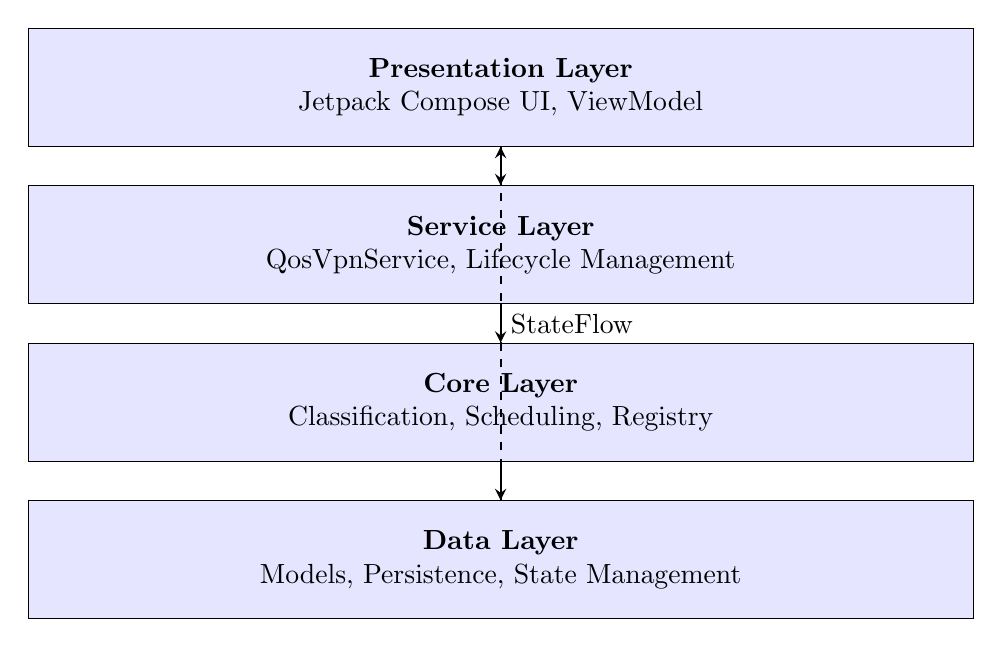
\begin{tikzpicture}[
    layer/.style={rectangle, draw, minimum width=12cm, minimum height=1.5cm, align=center, fill=blue!10},
    component/.style={rectangle, draw, minimum width=3cm, minimum height=1cm, align=center, fill=white},
    arrow/.style={->, >=stealth, thick}
]
    % Layers
    \node[layer] (ui) at (0,0) {\textbf{Presentation Layer}\\Jetpack Compose UI, ViewModel};
    \node[layer] (service) at (0,-2) {\textbf{Service Layer}\\QosVpnService, Lifecycle Management};
    \node[layer] (core) at (0,-4) {\textbf{Core Layer}\\Classification, Scheduling, Registry};
    \node[layer] (data) at (0,-6) {\textbf{Data Layer}\\Models, Persistence, State Management};
    
    % Arrows
    \draw[arrow] (ui) -- (service);
    \draw[arrow] (service) -- (core);
    \draw[arrow] (core) -- (data);
    \draw[arrow, dashed] (data) -- (ui) node[midway, right] {StateFlow};
\end{tikzpicture}
\caption{Four-Layer System Architecture}
\label{fig:system-architecture}
\end{figure}

\section{Component Specifications}
\label{sec:components}

\subsection{QosVpnService: Packet Interception and Forwarding}

The \code{QosVpnService} component is the system's core, responsible for:
\begin{itemize}
    \item Establishing and managing the TUN interface
    \item Reading raw packets from the tunnel
    \item Coordinating classification and scheduling
    \item Writing processed packets back to the tunnel
\end{itemize}

\subsubsection{Packet Processing Pipeline}

Algorithm~\ref{alg:packet-pipeline} formalizes the packet processing workflow.

\begin{algorithm}[htbp]
\caption{Packet Processing Pipeline}
\label{alg:packet-pipeline}
\begin{algorithmic}[1]
\Require TUN interface $T$, Classifier $C$, Scheduler $S$, Registry $R$
\Ensure Packets are classified, scheduled, and forwarded
\Procedure{ProcessPacket}{$rawBytes$, $length$}
    \State $packet \gets$ \Call{ParsePacket}{$rawBytes$, $length$}
    \If{$packet = \text{null}$}
        \State \Return \Comment{Malformed packet, drop silently}
    \EndIf
    
    \State $device \gets R.$\Call{GetOrCreate}{$packet.srcIp$}
    \State $R.$\Call{UpdateStats}{$packet.srcIp$, $length$}
    
    \State $category \gets C.$\Call{Classify}{$packet$}
    \State $flowKey \gets$ \Call{MakeFlowKey}{$packet$}
    \State $device.flows[flowKey].$\Call{Update}{$category$, $length$}
    
    \State $allowed \gets S.$\Call{ProcessPacket}{$packet$}
    \If{$allowed$}
        \State \Call{Write}{$T$, $rawBytes$, $length$}
        \State \Return \textsc{Forwarded}
    \Else
        \State \Return \textsc{Dropped}
    \EndIf
\EndProcedure
\end{algorithmic}
\end{algorithm}

\subsubsection{Rebalancing Strategy}

Bandwidth rebalancing is triggered by topology changes (device join/leave, priority change) rather than per-packet, reducing CPU overhead by $>90\%$.

\begin{algorithm}[htbp]
\caption{Conditional Rebalancing}
\label{alg:rebalancing}
\begin{algorithmic}[1]
\State $needsRebalance \gets \text{false}$
\State $packetCount \gets 0$
\Procedure{OnDeviceJoin}{$device$}
    \State $needsRebalance \gets \text{true}$
\EndProcedure
\Procedure{OnPriorityChange}{$device$, $newPriority$}
    \State $needsRebalance \gets \text{true}$
\EndProcedure
\Procedure{OnPacketProcessed}{}
    \State $packetCount \gets packetCount + 1$
    \If{$needsRebalance$ \textbf{or} $packetCount \bmod 1000 = 0$}
        \State \Call{Rebalance}{}
        \State $needsRebalance \gets \text{false}$
    \EndIf
\EndProcedure
\end{algorithmic}
\end{algorithm}

\subsection{DpiClassifier: Traffic Classification}

The \code{DpiClassifier} implements port-based classification with flow caching.

\subsubsection{Classification Rules}

Table~\ref{tab:classification-rules} defines the port-to-category mapping.

\begin{table}[htbp]
\centering
\caption{Traffic Classification Rules}
\label{tab:classification-rules}
\small
\begin{tabular}{@{}llll@{}}
\toprule
\textbf{Category} & \textbf{Protocol} & \textbf{Ports} & \textbf{Priority} \\
\midrule
Video Conferencing & UDP & 3478, 19302–19309 & HIGH \\
Video Conferencing & TCP & 443 (heuristic) & HIGH \\
Online Gaming & UDP & 27015–27030, 3074 & HIGH \\
Online Gaming & TCP & 25565 (Minecraft) & HIGH \\
VoIP & UDP & 5060, 5061, 16384–32767 & HIGH \\
Web Browsing & TCP & 80, 443 & MEDIUM \\
Streaming & TCP & 1935 (RTMP) & MEDIUM \\
File Transfer & TCP & 20, 21, 22, 445, 2049 & LOW \\
OS Updates & TCP & 80, 443 (heuristic) & LOW \\
Unknown & Any & Any & MEDIUM \\
\bottomrule
\end{tabular}
\end{table}

\subsubsection{Flow Caching}

To avoid re-classifying every packet of the same flow, we maintain a cache:

\begin{definition}[Flow Cache]
A flow cache $\mathcal{F}$ is a mapping from flow keys to categories:
\begin{equation}
\mathcal{F}: \text{FlowKey} \to \text{TrafficCategory}
\end{equation}
where $\text{FlowKey} = (srcIp, dstIp, srcPort, dstPort, protocol)$.

Cache lookup is $O(1)$ via hash table. Stale entries (no packets for $>30$ seconds) are evicted periodically.
\end{definition}

\subsection{BandwidthScheduler: Token Bucket Enforcement}

The \code{BandwidthScheduler} maintains per-device token buckets and implements weighted fair queuing.

\subsubsection{Token Bucket Formulation}

\begin{definition}[Per-Device Token Bucket]
For device $d$ with priority class $p \in \{\text{HIGH}, \text{MEDIUM}, \text{LOW}\}$, the token bucket $B_d$ is defined by:
\begin{align}
r_d &= C \cdot \frac{w_p}{\sum_{i=1}^{n} w_{p_i}} \label{eq:rate} \\
b_d &= \alpha_p \cdot r_d \label{eq:burst}
\end{align}
where:
\begin{itemize}
    \item $C$ is the total uplink capacity (bytes/second)
    \item $w_p$ is the weight for priority $p$ (HIGH=4, MEDIUM=2, LOW=1)
    \item $n$ is the number of connected devices
    \item $\alpha_p$ is the burst multiplier (HIGH=2, MEDIUM=1, LOW=0.5)
\end{itemize}
\end{definition}

\subsubsection{Token Refill and Consumption}

Algorithm~\ref{alg:token-bucket} implements the token bucket logic.

\begin{algorithm}[htbp]
\caption{Token Bucket Operations}
\label{alg:token-bucket}
\begin{algorithmic}[1]
\State $\tau \gets b$ \Comment{Initial tokens = burst capacity}
\State $t_{last} \gets$ \Call{CurrentTime}{}
\Procedure{Refill}{}
    \State $t_{now} \gets$ \Call{CurrentTime}{}
    \State $\Delta t \gets (t_{now} - t_{last}) / 10^9$ \Comment{Convert nanoseconds to seconds}
    \State $\tau \gets \min(b, \tau + r \cdot \Delta t)$
    \State $t_{last} \gets t_{now}$
\EndProcedure
\Procedure{Consume}{$packetSize$}
    \State \Call{Refill}{}
    \If{$\tau \geq packetSize$}
        \State $\tau \gets \tau - packetSize$
        \State \Return \textsc{Allowed}
    \Else
        \State \Return \textsc{Dropped}
    \EndIf
\EndProcedure
\end{algorithmic}
\end{algorithm}

\subsubsection{Weighted Fair Queuing Implementation}

When devices join or leave, or priorities change, we recompute token bucket rates:

\begin{algorithm}[htbp]
\caption{Weighted Fair Queuing Rebalance}
\label{alg:wfq-rebalance}
\begin{algorithmic}[1]
\Require Set of devices $D = \{d_1, \ldots, d_n\}$, uplink capacity $C$
\Ensure Token bucket rates updated for all devices
\Procedure{Rebalance}{$D$, $C$}
    \State $W \gets \sum_{i=1}^{n} w_{p_i}$ \Comment{Total weight}
    \For{each device $d_i \in D$}
        \If{$d_i$ has manual cap}
            \State $r_i \gets$ manual cap
        \Else
            \State $r_i \gets C \cdot \frac{w_{p_i}}{W}$
        \EndIf
        \State $b_i \gets \alpha_{p_i} \cdot r_i$
        \State $B_i.$\Call{SetRate}{$r_i$}
        \State $B_i.$\Call{SetBurst}{$b_i$}
    \EndFor
\EndProcedure
\end{algorithmic}
\end{algorithm}

\subsection{DeviceRegistry: State Management}

The \code{DeviceRegistry} tracks connected devices, maintains statistics, and persists priority assignments.

\subsubsection{Device Lifecycle}

\begin{figure}[htbp]
\centering
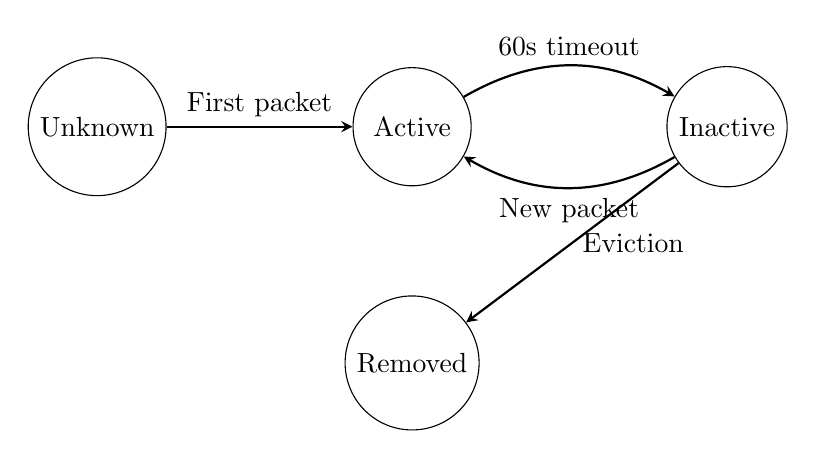
\begin{tikzpicture}[
    state/.style={circle, draw, minimum size=1.5cm, align=center},
    arrow/.style={->, >=stealth, thick}
]
    \node[state] (unknown) at (0,0) {Unknown};
    \node[state] (active) at (4,0) {Active};
    \node[state] (inactive) at (8,0) {Inactive};
    \node[state] (removed) at (4,-3) {Removed};
    
    \draw[arrow] (unknown) -- node[above] {First packet} (active);
    \draw[arrow] (active) to[bend left] node[above] {60s timeout} (inactive);
    \draw[arrow] (inactive) to[bend left] node[below] {New packet} (active);
    \draw[arrow] (inactive) -- node[right] {Eviction} (removed);
\end{tikzpicture}
\caption{Device Lifecycle State Machine}
\label{fig:device-lifecycle}
\end{figure}

\subsubsection{Throughput Sampling}

Real-time throughput is computed via a sliding window:

\begin{equation}
\theta_d(t) = \frac{B_d(t) - B_d(t - \Delta t)}{\Delta t}
\end{equation}

where $B_d(t)$ is the cumulative byte count for device $d$ at time $t$, and $\Delta t = 1$ second.

\subsubsection{Priority Persistence}

Device priorities are persisted using Android DataStore (Preferences API):

\begin{lstlisting}[language=Kotlin, caption={Priority Persistence}, label={lst:persistence}]
suspend fun persistPriority(mac: String, priority: TrafficClass) {
    val key = stringPreferencesKey("priority_$mac")
    dataStore.edit { preferences ->
        preferences[key] = priority.name
    }
}

suspend fun loadPersistedPriorities(): Map<String, TrafficClass> {
    return dataStore.data.first().asMap()
        .filter { it.key.name.startsWith("priority_") }
        .mapKeys { it.key.name.removePrefix("priority_") }
        .mapValues { TrafficClass.valueOf(it.value as String) }
}
\end{lstlisting}

\section{Data Flow Models}
\label{sec:data-flow}

\subsection{Packet Flow Sequence}

Figure~\ref{fig:packet-sequence} illustrates the complete packet processing sequence.

\begin{figure}[htbp]
\centering
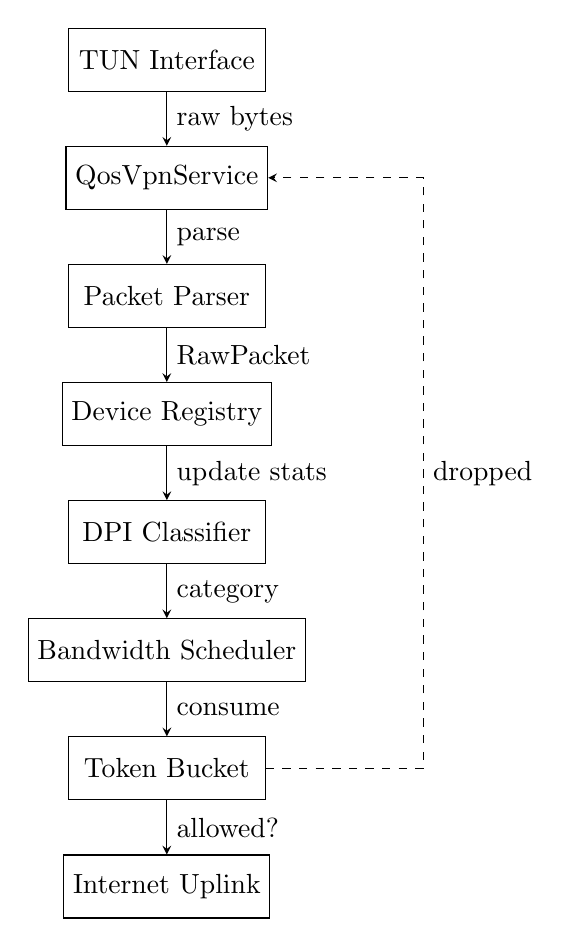
\begin{tikzpicture}[
    node distance=1.5cm,
    box/.style={rectangle, draw, minimum width=2.5cm, minimum height=0.8cm, align=center},
    arrow/.style={->, >=stealth}
]
    \node[box] (tun) {TUN Interface};
    \node[box, below of=tun] (vpn) {QosVpnService};
    \node[box, below of=vpn] (parser) {Packet Parser};
    \node[box, below of=parser] (registry) {Device Registry};
    \node[box, below of=registry] (classifier) {DPI Classifier};
    \node[box, below of=classifier] (scheduler) {Bandwidth Scheduler};
    \node[box, below of=scheduler] (bucket) {Token Bucket};
    \node[box, below of=bucket] (uplink) {Internet Uplink};
    
    \draw[arrow] (tun) -- node[right] {raw bytes} (vpn);
    \draw[arrow] (vpn) -- node[right] {parse} (parser);
    \draw[arrow] (parser) -- node[right] {RawPacket} (registry);
    \draw[arrow] (registry) -- node[right] {update stats} (classifier);
    \draw[arrow] (classifier) -- node[right] {category} (scheduler);
    \draw[arrow] (scheduler) -- node[right] {consume} (bucket);
    \draw[arrow] (bucket) -- node[right] {allowed?} (uplink);
    \draw[arrow, dashed] (bucket.east) -- ++(2,0) |- node[near start, right] {dropped} (vpn.east);
\end{tikzpicture}
\caption{Packet Processing Sequence Diagram}
\label{fig:packet-sequence}
\end{figure}

\subsection{Reactive State Propagation}

The system employs a reactive architecture where state changes propagate automatically:

\begin{equation}
\text{DeviceRegistry.devicesFlow} \xrightarrow{\text{collect}} \text{QosApplication.updateDevices} \xrightarrow{\text{combine}} \text{ViewModel.uiState} \xrightarrow{\text{observe}} \text{UI recompose}
\end{equation}

This eliminates manual state synchronization and ensures UI consistency.

\section{Interface Definitions}
\label{sec:interfaces}

\subsection{Classifier Interface}

\begin{lstlisting}[language=Kotlin, caption={Classifier Interface}, label={lst:classifier-interface}]
interface TrafficClassifier {
    fun classify(packet: RawPacket): TrafficCategory
    fun evictFlow(key: FlowKey)
    fun clearCache()
}
\end{lstlisting}

\subsection{Scheduler Interface}

\begin{lstlisting}[language=Kotlin, caption={Scheduler Interface}, label={lst:scheduler-interface}]
interface BandwidthScheduler {
    fun processPacket(packet: RawPacket): Boolean
    fun addDevice(device: ConnectedDevice)
    fun removeDevice(ipAddress: String)
    fun updatePriority(ipAddress: String, priority: TrafficClass)
    fun setManualCap(ipAddress: String, rateBps: Long)
    fun rebalanceWithDevices(devices: List<ConnectedDevice>)
}
\end{lstlisting}

\section{Performance Considerations}
\label{sec:performance-design}

\subsection{Critical Path Optimization}

The packet processing critical path (TUN read → parse → classify → schedule → TUN write) must complete in $<5$ ms. Optimizations include:

\begin{itemize}[leftmargin=*]
    \item \textbf{Zero-copy parsing:} \code{ByteBuffer.wrap()} avoids array copying
    \item \textbf{Flow cache:} $O(1)$ classification lookup for known flows
    \item \textbf{Lock-free reads:} \code{ConcurrentHashMap} enables concurrent device lookups
    \item \textbf{Nanosecond timing:} \code{System.nanoTime()} for precise token refill
\end{itemize}

\subsection{Memory Management}

To prevent memory leaks:
\begin{itemize}
    \item Flow cache entries expire after 30 seconds of inactivity
    \item Devices are evicted after 60 seconds of inactivity
    \item Packet buffers are reused (single 32KB allocation per service instance)
\end{itemize}

\subsection{Concurrency Model}

\begin{itemize}
    \item Packet loop runs on a dedicated coroutine (Dispatchers.IO)
    \item Device registry operations use \code{ConcurrentHashMap}
    \item Token bucket operations are \code{@Synchronized}
    \item UI updates propagate via \code{StateFlow} (thread-safe by design)
\end{itemize}

\section{Security and Privacy}
\label{sec:security-design}

\subsection{Privacy-Preserving Design}

\begin{itemize}
    \item \textbf{No payload logging:} Only packet headers (IP, port, protocol) are inspected
    \item \textbf{Local-only tunnel:} No traffic routed to external servers
    \item \textbf{Encrypted storage:} DataStore uses Android's encrypted preferences
    \item \textbf{No analytics:} No telemetry or usage data collection
\end{itemize}

\subsection{Threat Model}

\textbf{In-scope threats:}
\begin{itemize}
    \item Malicious client devices attempting to exhaust host resources
    \item Malformed packets causing parser crashes
\end{itemize}

\textbf{Out-of-scope threats:}
\begin{itemize}
    \item Compromised Android OS or kernel
    \item Physical access to the device
    \item Side-channel attacks on encrypted traffic
\end{itemize}

\section{Summary}

This chapter presented the complete system architecture:
\begin{itemize}
    \item Four-layer architecture with clear separation of concerns
    \item Detailed component specifications with algorithmic formulations
    \item Token bucket and weighted fair queuing implementations
    \item Reactive state management via Kotlin StateFlow
    \item Performance optimizations for sub-5ms packet processing
    \item Privacy-preserving design with no payload inspection
\end{itemize}

The next chapter discusses implementation details and Android-specific considerations.
